\documentclass{article}

\usepackage{fancyhdr} % Required for custom headers
\usepackage{lastpage} % Required to determine the last page for the footer
\usepackage{extramarks} % Required for headers and footers
\usepackage[usenames,dvipsnames]{color} % Required for custom colors
\usepackage{graphicx} % Required to insert images
\usepackage{listings} % Required for insertion of code
\usepackage{courier} % Required for the courier font
\usepackage{lipsum} % Used for inserting dummy 'Lorem ipsum' text into the template
\usepackage{amsmath}
\usepackage{amsthm}
\usepackage{amsfonts}
\usepackage{tikz}

\usetikzlibrary{automata,positioning}

% Margins
\topmargin=-0.45in
\evensidemargin=0in
\oddsidemargin=0in
\textwidth=6.5in
\textheight=9.0in
\headsep=0.25in

\linespread{1.1} % Line spacing

% Set up the header and footer
\pagestyle{fancy}
\lhead{\hmwkAuthorName} % Top left header
\chead{\hmwkClass\ (\hmwkClassInstructor\ \hmwkClassTime): \hmwkTitle} % Top center head
\rhead{\firstxmark} % Top right header
\lfoot{\lastxmark} % Bottom left footer
\cfoot{} % Bottom center footer
\rfoot{Page\ \thepage\ of\ \protect\pageref{LastPage}} % Bottom right footer
\renewcommand\headrulewidth{0.4pt} % Size of the header rule
\renewcommand\footrulewidth{0.4pt} % Size of the footer rule

\setlength\parindent{0pt} % Removes all indentation from paragraphs

%----------------------------------------------------------------------------------------
%	CODE INCLUSION CONFIGURATION
%----------------------------------------------------------------------------------------

\definecolor{MyDarkGreen}{rgb}{0.0,0.4,0.0} % This is the color used for comments
\lstloadlanguages{Perl} % Load Perl syntax for listings, for a list of other languages supported see: ftp://ftp.tex.ac.uk/tex-archive/macros/latex/contrib/listings/listings.pdf
\lstset{language=Perl, % Use Perl in this example
        frame=single, % Single frame around code
        basicstyle=\small\ttfamily, % Use small true type font
        keywordstyle=[1]\color{Blue}\bf, % Perl functions bold and blue
        keywordstyle=[2]\color{Purple}, % Perl function arguments purple
        keywordstyle=[3]\color{Blue}\underbar, % Custom functions underlined and blue
        identifierstyle=, % Nothing special about identifiers                                         
        commentstyle=\usefont{T1}{pcr}{m}{sl}\color{MyDarkGreen}\small, % Comments small dark green courier font
        stringstyle=\color{Purple}, % Strings are purple
        showstringspaces=false, % Don't put marks in string spaces
        tabsize=5, % 5 spaces per tab
        %
        % Put standard Perl functions not included in the default language here
        morekeywords={rand},
        %
        % Put Perl function parameters here
        morekeywords=[2]{on, off, interp},
        %
        % Put user defined functions here
        morekeywords=[3]{test},
       	%
        morecomment=[l][\color{Blue}]{...}, % Line continuation (...) like blue comment
        numbers=left, % Line numbers on left
        firstnumber=1, % Line numbers start with line 1
        numberstyle=\tiny\color{Blue}, % Line numbers are blue and small
        stepnumber=5 % Line numbers go in steps of 5
}

%----------------------------------------------------------------------------------------
%	DOCUMENT STRUCTURE COMMANDS
%	Skip this unless you know what you're doing
%----------------------------------------------------------------------------------------

% Header and footer for when a page split occurs within a problem environment
\newcommand{\enterProblemHeader}[1]{
\nobreak\extramarks{#1}{#1 continued on next page\ldots}\nobreak
\nobreak\extramarks{#1 (continued)}{#1 continued on next page\ldots}\nobreak
}

% Header and footer for when a page split occurs between problem environments
\newcommand{\exitProblemHeader}[1]{
\nobreak\extramarks{#1 (continued)}{#1 continued on next page\ldots}\nobreak
\nobreak\extramarks{#1}{}\nobreak
}

\setcounter{secnumdepth}{0} % Removes default section numbers
\newcounter{homeworkProblemCounter} % Creates a counter to keep track of the number of problems

\newcommand{\homeworkProblemName}{}
\newenvironment{homeworkProblem}[1][Problem \arabic{homeworkProblemCounter}]{ % Makes a new environment called homeworkProblem which takes 1 argument (custom name) but the default is "Problem #"
\stepcounter{homeworkProblemCounter} % Increase counter for number of problems
\renewcommand{\homeworkProblemName}{#1} % Assign \homeworkProblemName the name of the problem
\section{\homeworkProblemName} % Make a section in the document with the custom problem count
\enterProblemHeader{\homeworkProblemName} % Header and footer within the environment
}{
\exitProblemHeader{\homeworkProblemName} % Header and footer after the environment
}

\newcommand{\problemAnswer}[1]{ % Defines the problem answer command with the content as the only argument
\noindent\framebox[\columnwidth][c]{\begin{minipage}{0.98\columnwidth}#1\end{minipage}} % Makes the box around the problem answer and puts the content inside
}

\newcommand{\homeworkSectionName}{}
\newenvironment{homeworkSection}[1]{ % New environment for sections within homework problems, takes 1 argument - the name of the section
\renewcommand{\homeworkSectionName}{#1} % Assign \homeworkSectionName to the name of the section from the environment argument
\subsection{\homeworkSectionName} % Make a subsection with the custom name of the subsection
\enterProblemHeader{\homeworkProblemName\ [\homeworkSectionName]} % Header and footer within the environment
}{
\enterProblemHeader{\homeworkProblemName} % Header and footer after the environment
}

%----------------------------------------------------------------------------------------
%	NAME AND CLASS SECTION
%----------------------------------------------------------------------------------------

\newcommand{\hmwkTitle}{Homework\ \#1} % Assignment title
\newcommand{\hmwkDueDate}{January\ 31,\ 2012 at 11:59pm} % Due date
\newcommand{\hmwkClass}{CS331} % Course/class
\newcommand{\hmwkClassTime}{9:00am} % Class/lecture time
\newcommand{\hmwkClassInstructor}{Professor Zhang} % Teacher/lecturer
\newcommand{\hmwkAuthorName}{Josh Davis} % Your name

%----------------------------------------------------------------------------------------
%	TITLE PAGE
%----------------------------------------------------------------------------------------

\title{
\vspace{2in}
\textmd{\textbf{\hmwkClass:\ \hmwkTitle}}\\
\normalsize\vspace{0.1in}\small{Due\ on\ \hmwkDueDate}\\
\vspace{0.1in}\large{\textit{\hmwkClassInstructor\ \hmwkClassTime}}
\vspace{3in}
}

\author{\textbf{\hmwkAuthorName}}
\date{\today} % Insert date here if you want it to appear below your name

%----------------------------------------------------------------------------------------

\begin{document}

\maketitle
\pagebreak

\begin{homeworkProblem}
        Show that for any integer \(k \geq 2\), \(\sqrt[k]{2}\) is an irrational number.  \\\\
    \begin{proof}
        To prove by contradiction, suppose that \(\sqrt[k]{2}\) is rational. Then
        \[
            \sqrt[k]{2} = \frac{p}{q}
        \]

        where \(p\) and \(q\) are integers and co-prime. If we are to raise both sides to \(k\)
        then we get
        \[
            2 = \left(\frac{p}{q}\right)^k
        \]

        Which we can write as
        \[
            2 = \frac{p^k}{q^k}
        \]

        We multiply each side by \(q^k\) and get
        \[
            2q^k = p^k
        \]

        Thus \(p\) is even because any number times 2 is even. Let \(p = 2j\) for \(j \in \mathbb{Z}\). Then
        \[
            \begin{split}
                2q^k &= (2j)^k \\
                &= 2^k j^k
            \end{split}
        \]

        dividing both sides by 2 yields
        \[
            \begin{split}
                q^k &= 2^{k - 1} j^k \\
                q^k &= 2(2^{k - 2} j^k)
            \end{split}
        \]

        since \(k \geq 1\), \(q\) is even because any number multiplied by 2 is even. This is a contradiction
        because earlier \(p\) and \(q\) were co-prime meaning there were no numbers that could be divided
        into both of them. Thus \(p\) and \(q\) can't both be even.
    \end{proof}
\end{homeworkProblem}

\pagebreak

\begin{homeworkProblem}
        Show that for every \(n \geq 0\) a depth \(n\) perfect binary tree has \(2^{n+1} - 1\) nodes.  \\\\
    \begin{proof}
        We will do a proof by induction to prove that for every \(n \geq 0\) a perfect binary tree of has \(2^{n+1} - 1\) nodes.
        \\\\
        \textbf{Base} For the base case, we have a perfect binary tree of height \(= 0\). Then
        \[
            2^{n+1} - 1 = 2^{0 + 1} - 1 = 1 \mbox{ node}
        \]

        which is true because a tree of height 0 is a single root node.
        \\\\
        
        \textbf{Induction Step} We will prove that for every \(n \geq 0\) a perfect binary tree of height \(n + 1\) has \(2^{(n+1) + 1} - 1 \) nodes.
        \\
        Consider a tree, \(T\) with height \(h\). To create
        a perfect binary tree of height \(h + 1\), we can take two of \(T\) and connect
        it to a single root node. Thus
        \[
            \begin{split}
                \mbox{nodes} &= T + T + 1 \\
                &= 2T + 1
            \end{split}
        \]

        By the induction hypothesis
        \[
            \begin{split}
                \mbox{nodes} &= 2(2^{n+1} - 1) + 1 \\
                &= 2 \times 2^{n+1} - 2 + 1 \\
                &= 2 \times 2^{n+1} - 1 \\
                &= 2^{n + 2} - 1 \\
                &= 2^{(n + 1) + 1} - 1
            \end{split}
        \]

        Thus we have concluded our proof by showing that a perfect binary tree of height \(n + 1\) has \(2^{(n+1) + 1} - 1 \) nodes.
    \end{proof}
\end{homeworkProblem}

\pagebreak

\begin{homeworkProblem}

\end{homeworkProblem}

\pagebreak

\begin{homeworkProblem}
    Let \(\Sigma = \{0, 1\}\). What language is defined by the following regular expression? Define
    it in one or two sentences.
    \begin{enumerate}
        \item 
            \(\Sigma^{*} 0 \Sigma^{*} 1 \Sigma^{*}\) \\
            The language is the set of all words that have at least one 0 and one 1 in them.
        \item \(0 0^{*} 1^{*}\) \\
            The language is the set of all words that begin with a zero. The word also
            ends with any number of zeroes (including none) followed by any number of
            ones (including none).

    \end{enumerate}
\end{homeworkProblem}

\pagebreak

\begin{homeworkProblem}
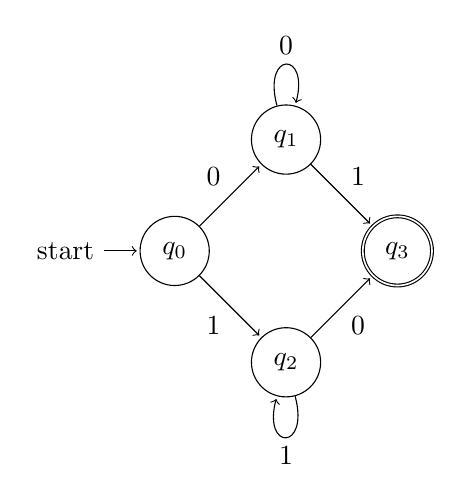
\begin{tikzpicture}[shorten >=1pt,node distance=2cm,on grid,auto] 
   \node[state,initial] (q_0)   {$q_0$}; 
   \node[state] (q_1) [above right=of q_0] {$q_1$}; 
   \node[state] (q_2) [below right=of q_0] {$q_2$}; 
   \node[state,accepting](q_3) [below right=of q_1] {$q_3$};
    \path[->] 
    (q_0) edge  node {0} (q_1)
          edge  node [swap] {1} (q_2)
    (q_1) edge  node  {1} (q_3)
          edge [loop above] node {0} ()
    (q_2) edge  node [swap] {0} (q_3) 
          edge [loop below] node {1} ();
\end{tikzpicture}
\end{homeworkProblem}

\pagebreak

\begin{homeworkProblem}

\end{homeworkProblem}

\end{document}
